%%
%% This is file `sample-sigconf.tex',
%% generated with the docstrip utility.
%%
%% The original source files were:
%%
%% samples.dtx  (with options: `sigconf')
%% 
%% IMPORTANT NOTICE:
%% 
%% For the copyright see the source file.
%% 
%% Any modified versions of this file must be renamed
%% with new filenames distinct from sample-sigconf.tex.
%% 
%% For distribution of the original source see the terms
%% for copying and modification in the file samples.dtx.
%% 
%% This generated file may be distributed as long as the
%% original source files, as listed above, are part of the
%% same distribution. (The sources need not necessarily be
%% in the same archive or directory.)
%%
%% The first command in your LaTeX source must be the \documentclass command.
\documentclass[sigconf, nonacm]{acmart}
\usepackage[english]{babel}
\usepackage{graphicx}
\usepackage{url}
\usepackage{multicol}
\usepackage{float}

% Table preamble
\usepackage{geometry}
\usepackage{changepage} % allows for temporary adjustment of side margins
\usepackage{xtab, array, booktabs, caption, ragged2e, lscape, threeparttablex}
% Redefine geometry commands
\makeatletter
\def\ifGm@preamble#1{\@firstofone}
\appto\restoregeometry{%
  \pdfpagewidth=\paperwidth
  \pdfpageheight=\paperheight}
\apptocmd\newgeometry{%
  \pdfpagewidth=\paperwidth
  \pdfpageheight=\paperheight}{}{}
\makeatother


%% NOTE that a single column version may be required for 
%% submission and peer review. This can be done by changing
%% the \doucmentclass[...]{acmart} in this template to 
%% \documentclass[manuscript,screen]{acmart}
%% 
%% To ensure 100% compatibility, please check the white list of
%% approved LaTeX packages to be used with the Master Article Template at
%% https://www.acm.org/publications/taps/whitelist-of-latex-packages 
%% before creating your document. The white list page provides 
%% information on how to submit additional LaTeX packages for 
%% review and adoption.
%% Fonts used in the template cannot be substituted; margin 
%% adjustments are not allowed.
%%
%%
%% \BibTeX command to typeset BibTeX logo in the docs
\AtBeginDocument{%
  \providecommand\BibTeX{{%
    \normalfont B\kern-0.5em{\scshape i\kern-0.25em b}\kern-0.8em\TeX}}}

%% Rights management information.  This information is sent to you
%% when you complete the rights form.  These commands have SAMPLE
%% values in them; it is your responsibility as an author to replace
%% the commands and values with those provided to you when you
%% complete the rights form.
\setcopyright{acmcopyright}
\copyrightyear{2020}
\acmYear{2020}


%%
%% Submission ID.
%% Use this when submitting an article to a sponsored event. You'll
%% receive a unique submission ID from the organizers
%% of the event, and this ID should be used as the parameter to this command.
%%\acmSubmissionID{123-A56-BU3}

%%
%% The majority of ACM publications use numbered citations and
%% references.  The command \citestyle{authoryear} switches to the
%% "author year" style.
%%
%% If you are preparing content for an event
%% sponsored by ACM SIGGRAPH, you must use the "author year" style of
%% citations and references.
%% Uncommenting
%% the next command will enable that style.
%%\citestyle{acmauthoryear}

%%
%% end of the preamble, start of the body of the document source.
\begin{document}

%%
%% The "title" command has an optional parameter,
%% allowing the author to define a "short title" to be used in page headers.
\title{A Conversational Agent for Math Tutoring}

%%
%% The "author" command and its associated commands are used to define
%% the authors and their affiliations.
%% Of note is the shared affiliation of the first two authors, and the
%% "authornote" and "authornotemark" commands
%% used to denote shared contribution to the research.
\author{Justin de Haan}
%\authornote{Both authors contributed equally to this research.}
\email{4623584}
\affiliation{%
  \institution{Delft University of Technology}
  \streetaddress{P.O. Box 1212}
  \city{Delft}
  \state{Zuid-Holland}
  \country{the Netherlands}
  \postcode{PO Box 5 2600 AA}
}

\author{Ynze ter Horst}
\email{4701682}
\affiliation{%
  \institution{Delft University of Technology}
  \streetaddress{P.O. Box 1212}
  \city{Delft}
  \state{Zuid-Holland}
  \country{the Netherlands}
  \postcode{PO Box 5 2600 AA}
}

\author{Marios Marinos}
\email{5353106}
\affiliation{%
  \institution{Delft University of Technology}
  \streetaddress{P.O. Box 1212}
  \city{Delft}
  \state{Zuid-Holland}
  \country{the Netherlands}
  \postcode{PO Box 5 2600 AA}
}

\author{Tim Polderdijk}
\email{4689313}
\affiliation{%
  \institution{Delft University of Technology}
  \streetaddress{P.O. Box 1212}
  \city{Delft}
  \state{Zuid-Holland}
  \country{the Netherlands}
  \postcode{PO Box 5 2600 AA}
}

%%
%% The abstract is a short summary of the work to be presented in the
%% article.
\begin{abstract}
  Numerous studies have been conducted to research learning environments. In this paper a conversational agent is introduced, which uses a range of techniques to automate and improve the learning experience of math students. The robot has functionalities to explain, train and test students to perform a rudimentary math skill. It also incorporates an emotion classifier to decide on an approach given the affective behaviour of the user.
\end{abstract}

%%
%% The code below is generated by the tool at http://dl.acm.org/ccs.cfm.
%% Please copy and paste the code instead of the example below.
%%
\begin{CCSXML}
<ccs2012>
<concept>
<concept_id>10003456.10003457.10003527</concept_id>
<concept_desc>Social and professional topics~Computing education</concept_desc>
<concept_significance>500</concept_significance>
</concept>
<concept>
<concept_id>10010405.10010489.10010495</concept_id>
<concept_desc>Applied computing~E-learning</concept_desc>
<concept_significance>500</concept_significance>
</concept>
</ccs2012>
\end{CCSXML}

\ccsdesc[500]{Social and professional topics~Computing education}
\ccsdesc[500]{Applied computing~E-learning}

%%
%% Keywords. The author(s) should pick words that accurately describe
%% the work being presented. Separate the keywords with commas.
\keywords{conversational agent, e-learning, emotion detection}

%% A "teaser" image appears between the author and affiliation
%% information and the body of the document, and typically spans the
%% page.
\begin{teaserfigure}
  
\includegraphics[width=\textwidth]{images/TU_delft_logo.jpg}
\end{teaserfigure}

%%
%% This command processes the author and affiliation and title
%% information and builds the first part of the formatted document.
\maketitle

\section{Introduction}
Math can be very challenging to master. Taking a personal approach to teaching is important to make sure the student stays engaged and dedicated to mastering the subject. We developed a conversational agent using the Furhat SDK \cite{Furhat} to teach a chosen math skill. Percentages is the math skill that we chose arbitrarily for this project, but that is not important for the purpose of the project and could have been any other math skill as well. The requirements for the agent were: that it has about 3 minutes of dialog flow to talk with the user, that there is some kind of gaze behavior implemented, and that it can detect the affect of the user (frustration for example). In this report we will document the design of our agent that achieves these requirements using affective computation and effective dialog management.\\

\noindent The goal of the agent is to teach a user a math skill while adapting to the emotional behaviour of the user, in this case mainly relating to the frustration and performance levels. The agent will guide the user through the process and tries to give the user a sense of achievement while doing so. Our agent is called Professor Euler. First it introduces itself and confirms with the user that they want to learn about percentages, then it has 2 different explanations, between which it can switch or repeat depending on the user's response. It also has different encouraging voicelines in case the user seems frustrated. After the agent is done with their explanation, it will ask some randomly generated exercises so the user can practice their newly learned skill. The agent keeps track of the users' score, so it can give a summary to the user when he/she is done. We also added some gestures to the agent's behavior to make it more human-like.
%% What is this report about? What are you trying to achieve?

\section{Motivation}
The approach to teaching has been extensively studied throughout the years. Irrespective of a lot of discourse in the field it has been widely established that affective behaviour plays a large role in the effectivity of a learning environment.\\

\noindent In \cite{shechtman2004affective} an extensive study was conducted, comparing a cognitive approach with an affective approach to teaching. Examples of results were a lesser frequency of misbehaviour, peer support, increased likelihood of expressing thoughts or feelings and more. Numerous studies like these have been performed and resulted in unambiguous results similar to the ones described above, examples are \cite{griffith2006educators} \cite{miller2005teaching} \cite{garritz2010personal}.\\

\noindent We think it is important for tutors to be emotionally involved in the process of guiding a student through the acquisition of a new, in this case mathematical, skill. It can be extremely frustrating when this process is cumbersome, especially for the student. The relevance of this project is exactly that, creating a conversational agent that doesn't trade in affection for automation but instead provides both.\\
%% Why does it make sense to create socially-aware dialog
%% systems? Where are possible application areas? (Please
%% include literature references here)

\section{Implementation}
In this section, we will go in into some of the implementation details of our math tutoring conversational agent. Specifically, we will discuss the data and architecture we have decided on using.

\subsection{Data}
\label{Data}
To be able to recognize the users' affective behaviour we used a pre-trained model\footnote{https://github.com/atulapra/Emotion-detection} that takes visual input using a camera, converts it to a 48x48 grayscale image and uses that to classify a range of 7 different emotions. The input is not saved during or after the emotion detection to make sure we don't harm the privacy of the user. We do not ask the user for any personal data for the same reason, as it is not required to teach math skill. Although we acknowledge that it could make the interactions more personalized.

\subsection{Architecture}
\label{Architecture}
Our bot is entirely built on an interaction framework called Furhat \cite{Furhat}; it provides extensive documentation and functionalities including gaze behaviour, gesturing, speech profiles, and more.\\

\noindent Furhat is mainly based on finite state transitions, so our systems architecture uses a rule-based approach to dialogue management. This design decision was mainly based on the robustness requirement we had for the bot, as the task can be modelled using a finite amount of states and we would like to stay in control of the tutor as to make sure the goal of the conversation is reached. Our dialogue flow is modelled in a UML format and can be found in appendix \ref{appendix:a}.\\

\noindent To make sure our conversational agent also has adaptive behaviour when it comes to both verbal and non-verbal input, we took a different approach than the rule-based one. As mentioned in the previous section we used machine learning principles instead, a convolutional neural network to be exact. The neural network classifies user emotion using visual input of the face of the user in real-time. These classified emotions are in turn used to determine the best approach in gazing, gesturing and even dialogue decisions to make sure the user has a constructive learning experience. In the figures below two examples are presented, showing the facial recognition and emotion classification in two different scenarios.

\begin{figure}[h]
\centering
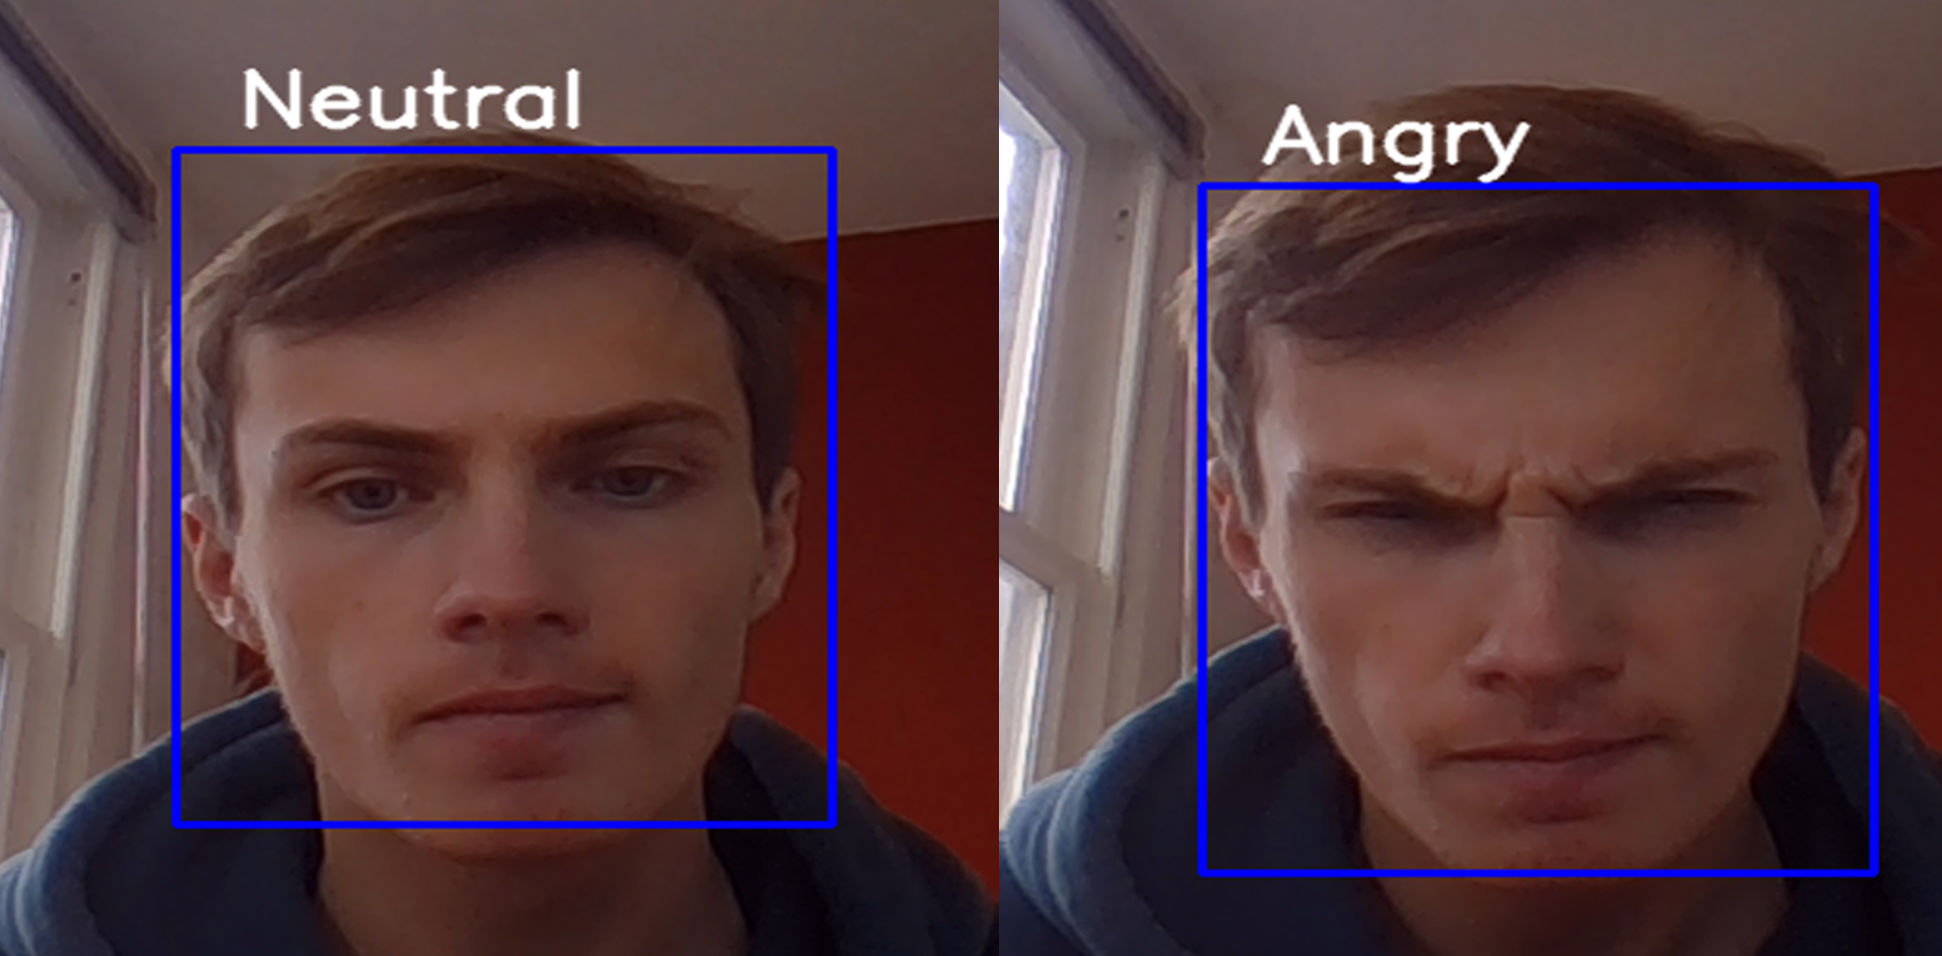
\includegraphics[width=\linewidth]{images/neutral_angry.png}
\caption{The classification of two affective behaviours}
\label{fig:emotion_detection}
\end{figure}

\subsection{Dialog flow}
The dialogue flow that we implemented for our agent can be found in appendix A. To create it we just imagined what a standard math teaching routine is like, and came up with dialogue lines that the tutor would say in that scenario. We separated them into 3 files in our project structure. The introduction and encouragement based on emotions are in mathtutor.kt, the explanations with examples are in explanation.kt, and the exercise questions (including generation) are in exercises.kt. We thought the agent was speaking a bit too fast during the explanations, so we changed the voice rate during those utterances to be 0.7. The agent has multiple possible lines it can say to encourage the user based on the detected emotion, and it randomly picks one of them each time it tries to encourage the user. This adds some variety to the dialogue and makes the agent seem more human-like. 

\subsection{Gaze behavior}
There are 3 types of gaze behavior which we could have implemented for our agent: random, rule-based, and data-driven. We immediately ruled out random because it would obviously be unreliable and probably very annoying from the user's perspective. In the end, we chose to use rule-based gaze behavior because it is much simpler to implement than creating a data-driven model, while it still achieves the desired effects with the right rules.
\newline
\newline
The two main gaze rules that we implemented are based on a research paper about the functions of gaze direction \cite{kendon1967some}. First, at the beginning of a long utterance, the agent should look away from the user. This gives the impression that the agent is still formulating the rest of what it is going to say. At the end of the utterance, it should look right at the user because it expects a response or reaction from the user. To implement this we made our agent look away for a few seconds at the start of long utterances and then look at the user after that. The location at which it looks away is chosen randomly from 4 points (up-left, up-right, down-left, down-right). We put extra pauses in the explanations during which the virtual agent glances away from the user as if the agent is preparing the next part of the explanation. When the agent continues, it just looks at the user again.
\newline
\newline
The other main rule we used is that the agent should look a bit lower than eye contact at the user for the beginning of long utterances, and end up looking into the users' eyes. To implement this rule we made it such that when our agent looks at the user during explanations, it looks slightly downwards, until asking the user for confirmation if they understood the explanation. For both of these rules we assume that the user is centered in front of the screen, at the same height as the agent. We had to use this assumption because we could not find where to get the location of the current user in Furhat.
\subsection{Gestures}
Gestures can potentially make the agent seem more human and we believe that will improve the user experience. That's why we decided to add some simple gesture behavior to the agent. By default, it wears a friendly smile towards the user. When the agent confirms an answer from the user to be correct it will put on a bigger smile and nod. If the user gives a wrong answer the agent will put away the smile while trying to console/encourage the user to make sure it is not perceived as laughing at the user for getting it wrong. After the exercise session, if the user got at least 60\% correct, it will show a bigger smile to them, then stop smiling after a second and ask the user if they want to practice more or not. If the user asks for help during the exercise session the agent will nod at them to confirm that it is going to help them.


\subsection{Emotion Detection}
The detect of emotion is very crucial when it comes in conversations involving humans interacting with humans. Many times, humans detect the emotions of the other speakers and intuitively they change their behaviour according to other's speaker feelings in order not to make them feel uncomfortable. Let's say that in a conversation between humans, one of them makes an inappropriate comment against the other and the other person feels sad. Then the person making the comment realizes that he said something wrong by seeing him sad, and feels sorry about it so he asks for forgiveness. Thus,  emotion detection is an essential part of our lives and plays a crucial role in how a conversation progresses.
\newline
\newline
Taking into consideration everything that has been said, it is evident that is very important for a conversational agent to be able to capture the emotions of the user to have a real conversation. The script that was used to detect the emotion of the user, is written in python using the pre-trained model which was mentioned in section \ref{Data}. The classes of the pre-trained model are 7: \{Angry, Disgusted, Happy, Neutral, Sad, Fearful, Surprised\}. Then, after the emotion has been detected, it is sent to a web-server (localhost:5000) where our agent parses the result and "combines" it with the user responses to give its reply. Therefore, each time the agent needs to know the emotion of the user, it will make a request to the web-server. The web-server calls the Emotion Detection script to capture the user's face at that moment and outputs the detected emotion on the web-server. This output is then processed by the agent. It should be noted that an assumption has been made that when the program cannot detect any face the moment it was requested, it always returns Neutral. 

\subsection{Usage of Emotion Detector}
The emotion detector was mostly used during the explanations of the math skill (e.g. percentages), as we want to detect if the user understands the explanation given by the agent. The agent will comfort the user if needed. It will do so based on the users' utterances and detected emotion. 
For the same reasons, the emotion was also captured in states where the exercises are being provided and explained.
\newline
\newline
Let's consider as an example the state Explanation1 to get a feeling of how the emotion detection works in combination with the user's responses. Firstly, the agent starts by requesting the users' emotion and if it detects surprise \textbf{before} starting the explanation, it will gon on encouraging the user before continuing with the explanation. When the explanation is completed, the agent asks whether the student has understood the given explanation. If the user responses "Yes" or "No" it transitions to the next states \textbf{without} checking his emotions. We have chosen this because the agents' main priority should be what the user said, regardless of what emotion has been detected. This is done for two reasons. Firstly, in real life, people tend to rely more on what the speaker is saying as this conveys more information and your detected emotion could be misjudged. Secondly, our emotion detector is not accurate enough to confidently rely on the detected emotion. 
If a user requests a "Repeat", the agent will detect the user's emotion and gives a motivational speech based on the detected emotion. Similarly, if a user responds with "do not know" or "do not understand", the agent detects the emotion and moves to the appropriate state. A diagram of this process is shown in appendix \ref{appendix:a}.
%% Data: Which data did you use in your implementation?
%% System -Architecture: How does your system architecture look like? Give reasons for the choices you made?

\section{Evaluation}
A controlled experiment has been performed to evaluate the user's perception of the virtual agent. This section will outline the methodology of this experiment and evaluate its outcome.

\subsection{Methodology}
\noindent 
To measure the social presence of the virtual agent, Harms et al. \cite{Alcaiz2004InternalCA} have developed a rigorous questionnaire covering social presence in six sub-dimensions.
To this end, one participant is recruited to interact with our virtual agent. The recruited participant has to be uninformed and unbiased towards the virtual agent. These requirements are necessary to obtain an objective evaluation of the user's perception, as anything less could affect the outcome of the questionnaire.
The virtual agent is provided to the participant on a computer set up by one of the researchers. Before the experiment is conducted, the participant has given their consent based on a modified online questionnaire template\footnote{https://www.tudelft.nl/en/about-tu-delft/strategy/integrity-policy/human-research-ethics/template-informed-consent-form/} created by the Human Research Ethics Committee of TU Delft.
After the participant finishes their interaction with the virtual agent, the previously mentioned questionnaire will be given to the participant to complete.

%To make sure we created an unbiased testing environment, we had to be careful about the recruitment of a participant. We made sure that the participant that would be testing our agent did not have any involvement whatsoever in the process of creating it. This was an important requirement because this not being the case could result in there being a bias towards functionalities of which flaws have been discovered in the development process, which might not be disruptive of the learning environment or show at all. Similarly, it might be the case that the opposite happens to such a participant, their hard work in a component of the system could for instance create a bias towards scoring these components higher. This meant we could not use a team member or a person that is doing or has done the same project. To this end we recruited a close relative of one of our team members to try out our setup.\\

%\noindent For the setup itself we installed our entire software package and asked the participant to go through a conversation with our agent. Afterwards, the participant was asked to fill in a questionnaire. This form is called the "Social Presence Evaluation", and provides a subjective measure to score conversational interactions on various dimensions.

\subsection{Results}
The table in appendix \ref{appendix:b} shows the questionnaire completed by our participant. The questionnaire uses a seven-point Likert-scale to measure each item. Response levels are mapped to consecutive integers from one to seven, where a score of 4 denotes the neutral middle. An average score per sub-dimension is calculated for further analysis. Questions 7, 8, 11, 12, 17, 18, 21, 22 has their score reversed to account for the negative phrasing in the question. For example, a score of 1 will become a score of 7 for these questions.
Table \ref{tab:results} shows the average score of each sub-dimension of the questionnaire. 

\begin{table}[h]
\centering
\begin{tabular}{@{}lcc@{}}
\toprule
Sub-Dimension                        & Formula                           & Score \\ \midrule
Co-Presence                          & $\frac{6 + 5 + 6 + 5 + 7 + 4}{6}$ & 5.5    \\\addlinespace
Attentional Allocation               & $\frac{3 + 3 + 6 + 3 + 6 + 4}{6}$ & 4.2    \\\addlinespace
Perceived Message Understanding      & $\frac{2 + 5 + 5 + 1 + 3 + 1}{6}$ & 2.8    \\\addlinespace
Perceived Affective Understanding    & $\frac{4 + 2 + 3 + 2 + 2 + 2}{6}$ & 2.5    \\\addlinespace
Perceived Emotional Interdependence  & $\frac{2 + 1 + 2 + 6 + 2 + 2}{6}$ & 2.5    \\\addlinespace
Perceived Behavioral Interdependence & $\frac{4 + 5 + 6 + 5 + 5 + 4}{6}$ & 4.8   \\\addlinespace
\end{tabular}
\caption{Calculated average score per sub-dimension}
\label{tab:results}
\end{table}

The next subsections will give a definition of each sub-dimension as defined in \cite{Alcaiz2004InternalCA}, as well as an interpretation of the measured score for the virtual agent.

\subsubsection{Co-Presence}~\\ %invisible char for line break
Co-presence is the degree to which the observer believes he/she is not alone and secluded, their level of peripheral or focal awareness of the other, and their sense of the degree to which the other is peripherally or focally aware of them. 
An average score of 5.5 indicates that the participant agrees that the virtual agent and participant are focally aware of each other and not alone and secluded.

\subsubsection{Attentional Allocation}~\\
\label{sub:AttentionalAllocation}
Attentional allocation addresses the amount of attention the user allocates to and receives from an interactant.
An average score of 4.2 means that the participant feels neutral about the attentional allocation. Looking at each question in this dimension, it seems that the participant got slightly distracted as the virtual agent did not remain focused on the participant. A possible explanation for this will be given in the next subsection. 

\subsubsection{Perceived Message Understanding}~\\
Perceived message understanding is the ability of the user to understand the message being received from the interactant as well as their perception of the interactant’s level of message understanding.
The participant gave an average score of 2.8 for this dimension, which is below average. Looking at each individual item in this dimension, the participant was able to understand the virtual agent reasonably well. However, the virtual agent has a lot of trouble understanding the participant. The researchers observed that the speech interpreter sometimes didn't recognize the participant's speech, making the virtual agent ask the participant to repeat what was said. The participant then proceeded to repeat their utterances while the virtual agent was still talking, making the virtual agent unable to listen to their utterances and ask the participant to repeat again. This results in a low score for the virtual agent's level of message understanding. This issue could also explain the perceived loss of attention in subsection \ref{sub:AttentionalAllocation} as it seems the virtual agent is not listening to the participant.

\subsubsection{Perceived Affective Understanding}~\\
\label{sub:PerceivedAffective}
Perceived affective understanding is the user’s ability to understand an interactant’s emotional and attitudinal states as well as their perception of the interactant’s ability to understand the user’s emotional and attitudinal states. The score for this dimension is a 2.5, meaning that the participant and virtual agent did not understand each others emotions very well. This indicates that the system responsible for the virtual agent's emotions and its emotion detector did not work as expected.

\subsubsection{Perceived Emotional Interdependence}~\\
Perceived affective interdependence is the extent to which the user’s emotional and attitudinal state affects and is affected by the emotional and attitudinal states of the interactant. This dimension got an average score of 2.5. The average score is still relatively high because the participant agrees that their mood did influence the interaction for themselves. However, the participant didn't think their emotions and attitudinal state influenced the interaction with the virtual agent at all. As discussed in subsection \ref{sub:PerceivedAffective}, this is likely because the emotional detection system is not working as intended.

\subsubsection{Perceived Behavioral Interdependence}~\\
Perceived behavioral interdependence is the extent to which the participants behaviour affects and is affected by the interactant’s behavior. 
An average score of 4.8 means that the participant somewhat agrees to this statement. This score would probably improve if the emotion detection is working as intended, as it could respond better to the users' behavior.


%% Present your Questionnaire results here

\section{Discussion}
In retrospect, there are several aspects in our agent that we either thought could have had a better realisation or instead turned out very satisfactory. In this section, we will review the process of the development of our math tutoring agent, specifically what went according to plan and what ended up not living up to our expectations.\\

\noindent Let's start on the negative side of things. At the start of our project, we were very interested in incorporating emotion recognition for our agent to adapt its’ behaviour according to the users’ supposed emotion. This was very relevant for our context, as a main requirement for the tutor was its dynamic behaviour concerning the frustration of the user. In retrospect, it may have been too ambitious to find such a model that predicts these affects with an accuracy that is satisfying to that end. Instead, we found our model to often fall back to a neutral classification or not recognizing the face itself at all. The model we used was scored with a 63\% accuracy rate using annotated visual input.\\

\noindent A second aspect that turned out to make for a cumbersome experience was discovered in the evaluation phase. Since we as developers were supposedly unconsciously aware of this problem the issue did not reveal itself at an earlier stage. When our subject was interacting with the tutor it came to our attention that the number of retries due to unrecognized speech was significantly higher than we had experienced ourselves. This might be due to the subjects accent or otherwise the aforementioned hypothesis involving our unconscious avoidance of the problem.\\

\noindent There was another issue that was brought to the light in this evaluation. During the installation of all the different components of our system, we noticed that there were quite a lot of independent components needed specific software versions in order to integrate with the whole. To tackle this issue, we have written instructions to set up all different components.\\

\noindent Finally, let’s touch on some of the aspects that we are proud of. We think what makes our tutor so useful is that it essentially takes a process that could very simply be individualized and creates a tutoring experience around it. Apart from that, it is not just a math tutor but can be any kind of tutor as the source code is easily adaptable to incorporate new domain knowledge and even allows for migration to a completely different domain altogether. The robustness of the agent allows the initiative of the dialogue to stay with the agent and provides the possibility for a directed and focused approach to learning in this setting.
%% Limitations
%% a. What did not work and why do you think that is? 
%% b. What are the strengths of your system and where are the weaknesses.

\section{Conclusion}
% \newpage
% summarize results here
In summary, from the findings presented in the previous sections, a few interesting remarks can be made regarding the virtual agent.

Firstly, the virtual agent could be expanded to become a general math tutor that is capable of teaching more math skills, not only percentages. This would be a necessity if the virtual agent is to be used as an actual product, as the target audience is too small if it can only teach one skill. The explanation-exercise-feedback loop is already implemented and can be reused for other math skills. The dialogue flow would need to be expanded for new math skills and some additional states have to be added to let the user switch between math skills.

Secondly, the outcome of the evaluation shows that the emotion-detection system has to be revamped. One future direction could be to apply machine-learning on the users' utterances to give better encouragements based on the users' emotion. This would increase the perceived emotional interdependence. 

Another possibility is to capture the users' emotional and attitudinal states better than it's doing currently and let the virtual agent mirror them. An example of this could be to incorporate data like voice pitch and voice intensity. This would increase the perceived affective understanding between the virtual agent and the user. To increase the co-presence and attentional allocation of the virtual agent, it would be good if the virtual agent is capable of listening to users' utterances while speaking, or halt when the user is speaking. This would also increase the perceived message understanding of the virtual agent as the user doesn't have to repeat their utterances that much.
Overall, there is a lot of potential in this field of research in terms of real-world applications. The technology and research regarding virtual agents in e-learning will hopefully increase in the coming years such that these agents become a viable alternative to private tutors.
%% Summarize your results and give suggestions for future work

%%
%% The acknowledgments section is defined using the "acks" environment
%% (and NOT an unnumbered section). This ensures the proper
%% identification of the section in the article metadata, and the
%% consistent spelling of the heading.
\begin{acks}
% To Robert, for the bagels and explaining CMYK and color spaces.
\end{acks}

%%
%% The next two lines define the bibliography style to be used, and
%% the bibliography file.
\bibliographystyle{ACM-Reference-Format}
\bibliography{ref}

%%
%% If your work has an appendix, this is the place to put it.


\onecolumn
\appendix
\section{Diagram of explanation state}
\label{appendix:a}
\begin{figure}[H]
\centering
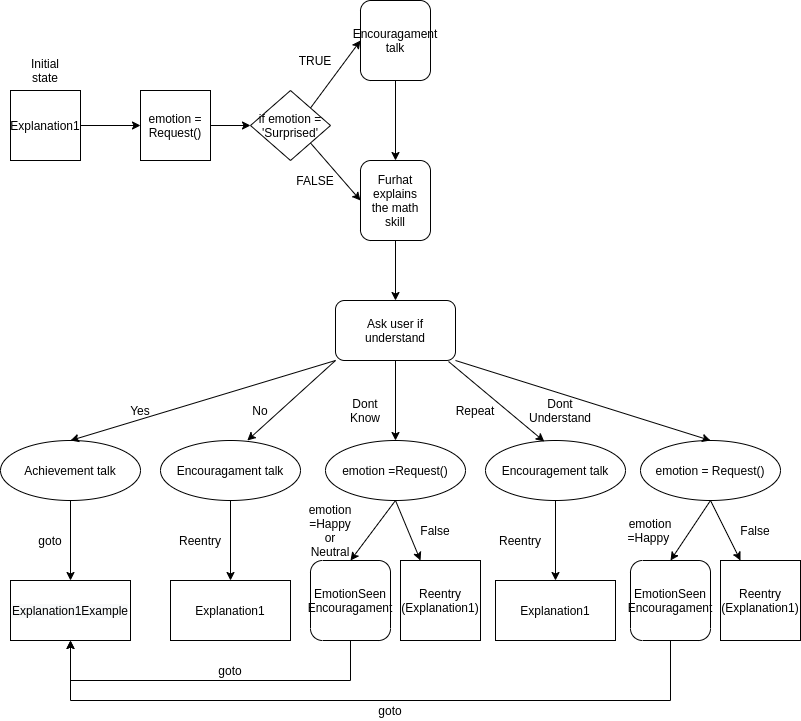
\includegraphics[width=\linewidth]{images/StateDiagram.png}
\caption{Diagram of state Explanation 1.}
\label{fig:State}
\end{figure}

\newpage
\section{Dialogue flow}
\label{appendix:b}
\begin{figure*}[h]
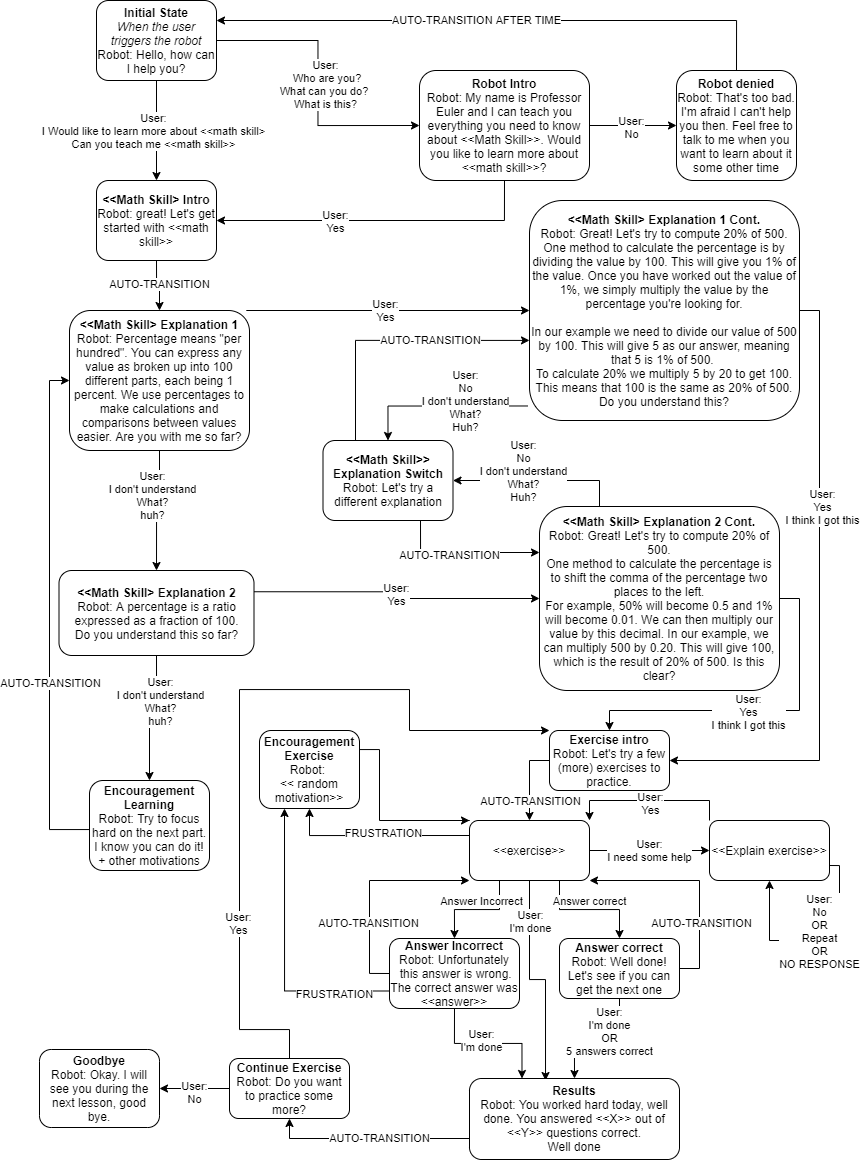
\includegraphics[width=\linewidth, height=0.9\textheight]{images/DialogFlow.png}
\caption{Dialog flow of the math skill tutorial}

\end{figure*}

% Please add the following required packages to your document preamble:
% \usepackage{booktabs}
% \usepackage{lscape}
\newgeometry{hmargin=0.4cm,vmargin=1.6cm,landscape}
% \onecolumn % use the full width of the page
\section{Social Presence Questionnaire Completed}
\label{appendix:c}
\begin{table}[h]
\centering
\begin{tabular}{@{}lcl|ccccccc@{}}
\toprule
Sub-Dimension                        & Question &                                                                            & \begin{tabular}[c]{@{}c@{}}Strongly \\ Disagree\end{tabular} & Disagree & \begin{tabular}[c]{@{}c@{}}Somewhat \\ Disagree\end{tabular} & Neutral & \begin{tabular}[c]{@{}c@{}}Somewhat \\ Agree\end{tabular} & Agree & \begin{tabular}[c]{@{}c@{}}Strongly \\ Agree\end{tabular} \\ \midrule
Co-Presence                          & 1.       & I noticed (my partner)                                                     &                                                              &          &                                                              &         &                                                           & X     &                                                           \\
                                     & 2.       & (My partner) noticed me                                                    &                                                              &          &                                                              &         & X                                                         &       &                                                           \\
                                     & 3.       & (My partner's) presence was obvious to me                                  &                                                              &          &                                                              &         &                                                           & X     &                                                           \\
                                     & 4.       & My presence was obvious to (my partner)                                    &                                                              &          &                                                              &         & X                                                         &       &                                                           \\
                                     & 5.       & (My partner) caught my attention                                           &                                                              &          &                                                              &         &                                                           &       & X                                                         \\
                                     & 6.       & I caught (my partner's) attention                                          &                                                              &          &                                                              & X       &                                                           &       &                                                           \\ \midrule
Attentional Allocation               & 7.       & I was easily distracted from (my partner) when other things were going on  &                                                              &          &                                                              &         & X                                                         &       &                                                           \\
                                     & 8.       & (My partner) was easily distracted from me when other things were going on &                                                              &          &                                                              &         & X                                                         &       &                                                           \\
                                     & 9.       & I remained focused on (my partner) throughout our interaction              &                                                              &          &                                                              &         &                                                           & X     &                                                           \\
                                     & 10.      & (My partner) remained focused on me throughout our interaction             &                                                              &          & X                                                            &         &                                                           &       &                                                           \\
                                     & 11.      & (My partner) did not receive my full attention                             &                                                              & X        &                                                              &         &                                                           &       &                                                           \\
                                     & 12.      & I did not receive (my partner's) full attention                            &                                                              &          &                                                              & X       &                                                           &       &                                                           \\ \midrule
Perceived Message Understanding      & 13.      & My thoughts were clear to (my partner)                                     &                                                              & X        &                                                              &         &                                                           &       &                                                           \\
                                     & 14.      & (My partner's) thoughts were clear to me                                   &                                                              &          &                                                              &         & X                                                         &       &                                                           \\
                                     & 15.      & It was easy to understand (my partner)                                     &                                                              &          &                                                              &         & X                                                         &       &                                                           \\
                                     & 16.      & (My partner) found it easy to understand me                                & X                                                            &          &                                                              &         &                                                           &       &                                                           \\
                                     & 17.      & Understanding (my partner) was difficult                                   &                                                              &          &                                                              &         & X                                                         &       &                                                           \\
                                     & 18.      & (My partner) had difficulty understanding me                               &                                                              &          &                                                              &         &                                                           &       & X                                                         \\ \midrule
Perceived Affective Understanding    & 19.      & I could tell how (my partner) felt                                         &                                                              &          &                                                              & X       &                                                           &       &                                                           \\
                                     & 20.      & (My partner) could tell how I felt                                         &                                                              & X        &                                                              &         &                                                           &       &                                                           \\
                                     & 21.      & (My partner's) emotions were not clear to me                               &                                                              &          &                                                              &         & X                                                         &       &                                                           \\
                                     & 22.      & My emotions were not clear to (my partner)                                 &                                                              &          &                                                              &         &                                                           & X     &                                                           \\
                                     & 23.      & I could describe (my partner's) feelings accurately                        &                                                              & X        &                                                              &         &                                                           &       &                                                           \\
                                     & 24.      & (My partner) could describe my feelings accurately                         &                                                              & X        &                                                              &         &                                                           &       &                                                           \\ \midrule
Perceived Emotional Interdependence  & 25.      & I was sometimes influenced by (my partner's) moods                         &                                                              & X        &                                                              &         &                                                           &       &                                                           \\
                                     & 26.      & (My partner) was sometimes influenced by my moods                          & X                                                            &          &                                                              &         &                                                           &       &                                                           \\
                                     & 27.      & (My partner's) feelings influenced the mood of our interaction             &                                                              & X        &                                                              &         &                                                           &       &                                                           \\
                                     & 28.      & My feelings influenced the mood of our interaction                         &                                                              &          &                                                              &         &                                                           & X     &                                                           \\
                                     & 29.      & (My partner's) attitudes influenced how I felt                             &                                                              & X        &                                                              &         &                                                           &       &                                                           \\
                                     & 30.      & My attitudes influenced how (my partner) felt                              &                                                              & X        &                                                              &         &                                                           &       &                                                           \\ \midrule
Perceived Behavioral Interdependence & 31.      & My behaviour was often in direct response to (my partner's) behaviour      &                                                              &          &                                                              & X       &                                                           &       &                                                           \\
                                     & 32.      & The behaviour of (my partner) was often in direct response to my behaviour &                                                              &          &                                                              &         & X                                                         &       &                                                           \\
                                     & 33.      & I reciprocated (my partner's) actions                                      &                                                              &          &                                                              &         &                                                           & X     &                                                           \\
                                     & 34.      & (My partner) reciprocated my actions                                       &                                                              &          &                                                              &         & X                                                         &       &                                                           \\
                                     & 35.      & (My partner's) behaviour was closely tied to my behaviour                  &                                                              &          &                                                              &         & X                                                         &       &                                                           \\
                                     & 36.      & My behaviour was closely tied to (my partner's) behaviour                  &                                                              &          &                                                              & X       &                                                           &       &                                                           \\ \bottomrule
\end{tabular}
% \caption{Result of evaluation}
\label{tab:evaluation}
\end{table}
\restoregeometry % restore normal page margins
% \subsection{Part One}
% \subsection{Part Two}
% \section{Online Resources}


\end{document}
\endinput